\documentclass[border=6pt]{standalone}
\usepackage{tikz}
\usetikzlibrary{arrows.meta,positioning,shapes.geometric,calc}
\begin{document}
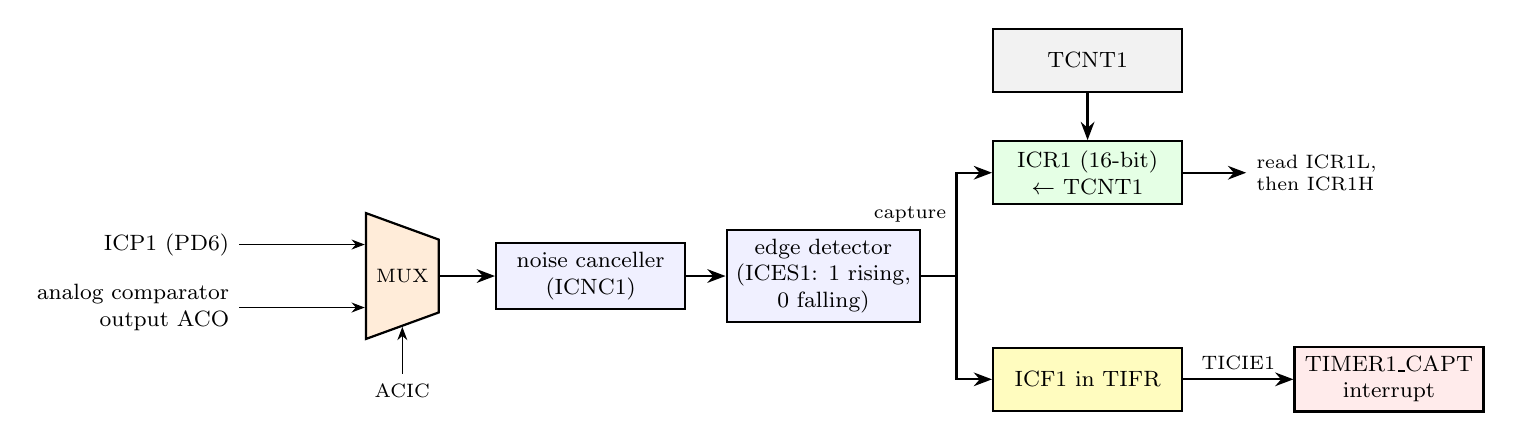
\begin{tikzpicture}[>=Stealth,font=\small,node distance=0.5cm,
 b/.style={draw,thick,fill=blue!6,align=center,font=\footnotesize,minimum height=0.8cm,minimum width=2.4cm}]
\node[draw,thick,fill=orange!15,trapezium,trapezium angle=70,shape border rotate=270,minimum height=0.8cm,minimum width=1.6cm] (mux) at (0,0) {};
\node[font=\scriptsize] at (0,0) {MUX};
\draw[<-] ($(mux.west)+(0,0.4)$) -- ++(-1.6,0) node[left,font=\footnotesize]{ICP1 (PD6)};
\draw[<-] ($(mux.west)+(0,-0.4)$) -- ++(-1.6,0) node[left,font=\footnotesize,align=right]{analog comparator\\output ACO};
\draw[<-] (mux.south) -- ++(0,-0.6) node[below,font=\scriptsize]{ACIC};
\node[b,right=0.7cm of mux] (nc) {noise canceller\\(ICNC1)};
\node[b,right=of nc] (ed) {edge detector\\(ICES1: 1 rising,\\0 falling)};
\draw[->,thick] (mux.east) -- (nc);
\draw[->,thick] (nc) -- (ed);
\node[b,fill=green!10,above right=0.3cm and 0.9cm of ed] (icr) {ICR1 (16-bit)\\$\leftarrow$ TCNT1};
\node[b,fill=yellow!25,below right=0.3cm and 0.9cm of ed] (icf) {ICF1 in TIFR};
\draw[->,thick] (ed.east) -- ++(0.45,0) |- (icr.west) node[pos=0.3,left,font=\scriptsize]{capture};
\draw[->,thick] (ed.east) -- ++(0.45,0) |- (icf.west);
\node[b,fill=gray!10,above=0.6cm of icr] (tc) {TCNT1};
\draw[->,thick] (tc) -- (icr);
\node[b,fill=red!8,right=1.4cm of icf] (irq) {TIMER1\_CAPT\\interrupt};
\draw[->,thick] (icf) -- (irq) node[midway,above,font=\scriptsize]{TICIE1};
\draw[->,thick] (icr.east) -- ++(0.8,0) node[right,font=\scriptsize,align=left]{read ICR1L,\\then ICR1H};
\end{tikzpicture}
\end{document}
